\documentclass[12pt, twoside, openright]{report} %fuente a 12pt, formato doble pagina y chapter a la derecha
\raggedbottom % No ajustar el contenido con un salto de pagina

% MÁRGENES: 2,5 cm sup. e inf.; 3 cm izdo. y dcho.
\usepackage[
a4paper,
vmargin=2.5cm,
hmargin=3cm
]{geometry}

% INTERLINEADO: Estrecho (6 ptos./interlineado 1,15) o Moderado (6 ptos./interlineado 1,5)
\renewcommand{\baselinestretch}{1.15}
\parskip=6pt

% DEFINICIÓN DE COLORES para portada y listados de código
\usepackage[table]{xcolor}
\definecolor{azulUC3M}{RGB}{0,0,102}
\definecolor{gray97}{gray}{.97}
\definecolor{gray75}{gray}{.75}
\definecolor{gray45}{gray}{.45}

% Soporte para GENERAR PDF/A
\usepackage[a-1b]{pdfx}

% ENLACES
\usepackage{hyperref}
\hypersetup{colorlinks=true,
	linkcolor=black, % enlaces a partes del documento (p.e. índice) en color negro
	urlcolor=blue} % enlaces a recursos fuera del documento en azul

% Añadir pdfs como partes del documento
\usepackage{pdfpages}

% Quitar la indentación de principio de los parrafos
\setlength{\parindent}{0em}

% EXPRESIONES MATEMATICAS
\usepackage{amsmath,amssymb,amsfonts,amsthm}

\usepackage{txfonts} 
\usepackage[T1]{fontenc}
\usepackage[utf8]{inputenc}

% Insertar graficas y fotos
\usepackage{tikz}
\usepackage{pgfplots}

\usepackage[spanish, es-tabla]{babel} 
\usepackage[babel, spanish=spanish]{csquotes}
\AtBeginEnvironment{quote}{\small}

% diseño de PIE DE PÁGINA
\usepackage{fancyhdr}
\pagestyle{fancy}
\fancyhf{}
\renewcommand{\headrulewidth}{0pt}
\fancyfoot[LE,RO]{\thepage}
\fancypagestyle{plain}{\pagestyle{fancy}}

% DISEÑO DE LOS TÍTULOS de las partes del trabajo (capítulos y epígrafes o subcapítulos)
\usepackage{titlesec}
\usepackage{titletoc}
\titleformat{\chapter}[block]
{\large\bfseries\filcenter}
{\thechapter.}
{5pt}
{\MakeUppercase}
{}
\titlespacing{\chapter}{0pt}{0pt}{*3}
\titlecontents{chapter}
[0pt]                                               
{}
{\contentsmargin{0pt}\thecontentslabel.\enspace\uppercase}
{\contentsmargin{0pt}\uppercase}                        
{\titlerule*[.7pc]{.}\contentspage}                 

\titleformat{\section}
{\bfseries}
{\thesection.}
{5pt}
{}
\titlecontents{section}
[5pt]                                               
{}
{\contentsmargin{0pt}\thecontentslabel.\enspace}
{\contentsmargin{0pt}}
{\titlerule*[.7pc]{.}\contentspage}

\titleformat{\subsection}
{\normalsize\bfseries}
{\thesubsection.}
{5pt}
{}
\titlecontents{subsection}
[10pt]                                               
{}
{\contentsmargin{0pt}                          
	\thecontentslabel.\enspace}
{\contentsmargin{0pt}}                        
{\titlerule*[.7pc]{.}\contentspage}  


% DISEÑO DE TABLAS.
\usepackage{multirow} % permite combinar celdas 
\usepackage{caption} % para personalizar el título de tablas y figuras
\usepackage{floatrow} % utilizamos este paquete y sus macros \ttabbox y \ffigbox para alinear los nombres de tablas y figuras de acuerdo con el estilo definido. Para su uso ver archivo de ejemplo 
\usepackage{array} % con este paquete podemos definir en la siguiente línea un nuevo tipo de columna para tablas: ancho personalizado y contenido centrado
\newcolumntype{P}[1]{>{\centering\arraybackslash}p{#1}}
\DeclareCaptionFormat{upper}{#1#2\uppercase{#3}\par}

% Diseño de tabla para ingeniería
\captionsetup[table]{
	format=hang,
	name=Tabla,
	justification=centering,
	labelsep=colon,
	width=.75\linewidth,
	labelfont=small,
	font=small,
}

% DISEÑO DE FIGURAS.
\usepackage{graphicx}
\graphicspath{{img/}} %ruta a la carpeta de imágenes

% Diseño de figuras para ingeniería
\captionsetup[figure]{
	format=hang,
	name=Fig.,
	singlelinecheck=off,
	labelsep=colon,
	labelfont=small,
	font=small		
}

% NOTAS A PIE DE PÁGINA
\usepackage{chngcntr} %para numeración continua de las notas al pie
\counterwithout{footnote}{chapter}

% LISTADOS DE CÓDIGO
% soporte y estilo para listados de código. Más información en https://es.wikibooks.org/wiki/Manual_de_LaTeX/Listados_de_código/Listados_con_listings
\usepackage{listings}

% definimos un estilo de listings
\lstdefinestyle{estilo}{ frame=Ltb,
	framerule=0pt,
	aboveskip=0.5cm,
	framextopmargin=3pt,
	framexbottommargin=3pt,
	framexleftmargin=0.4cm,
	framesep=0pt,
	rulesep=.4pt,
	backgroundcolor=\color{gray97},
	rulesepcolor=\color{black},
	%
	basicstyle=\ttfamily\footnotesize,
	keywordstyle=\bfseries,
	stringstyle=\ttfamily,
	showstringspaces = false,
	commentstyle=\color{gray45},     
	%
	numbers=left,
	numbersep=15pt,
	numberstyle=\tiny,
	numberfirstline = false,
	breaklines=true,
	xleftmargin=\parindent
}

\captionsetup[lstlisting]{font=small, labelsep=period}
% fijamos el estilo a utilizar 
\lstset{style=estilo}
\renewcommand{\lstlistingname}{\uppercase{Código}}

\pgfplotsset{compat=1.17} 
%-------------
%	DOCUMENTO
%-------------

\begin{document}
\pagenumbering{roman} % Se utilizan cifras romanas en la numeración de las páginas previas al cuerpo del trabajo
	
%----------
%	PORTADA
%----------	
\begin{titlepage}
	\begin{sffamily}
	\color{azulUC3M}
	\begin{center}
		\begin{figure}[H] %incluimos el logotipo de la Universidad
			\makebox[\textwidth][c]{
\includegraphics[width=16cm]{Portada_Logo.png}}
		\end{figure}
		\vspace{2.5cm}
		\begin{Large}
			Grado en Ingeniería Informática\\			
			2019-2020\\
			\vspace{2cm}		
			\textsl{Apuntes}\\
			\bigskip
		\end{Large}
		 	{\Huge Principios de desarrollo de software}\\
		 	\vspace*{0.5cm}
	 		\rule{10.5cm}{0.1mm}\\
			\vspace*{0.9cm}
			{\LARGE Jorge Rodríguez Fraile\footnote{\href{mailto:100405951@alumnos.uc3m.es}{Universidad: 100405951@alumnos.uc3m.es}  |  \href{mailto:jrf1616@gmail.com}{Personal: jrf1616@gmail.com}}}\\ 
			\vspace*{1cm}
	\end{center}
	\vfill
	\color{black}
		
\includegraphics[width=4.2cm]{img/creativecommons.png}\\
		Esta obra se encuentra sujeta a la licencia Creative Commons\\ \textbf{Reconocimiento - No Comercial - Sin Obra Derivada}
	\end{sffamily}
\end{titlepage}

%----------
%	ÍNDICES
%----------	

%--
% Índice general
%-
\tableofcontents
\thispagestyle{fancy}

%----------
%	TRABAJO
%----------	

\pagenumbering{arabic} % numeración con múmeros arábigos para el resto de la publicación	


%----------
%	COMENZAR A ESCRIBIR AQUI
%----------	



\part{Resúmenes}
\chapter{Tema 1: Aspectos éticos y profesionales relativos a la profesión
de la Ingeniería del Software.}

\begin{itemize}
\item El ingeniero de software es más parecido a un artesano que aun
  ingeniero.
\item \textbf{Ingeniero:} Aplica el \underline{método científico},
  resolviendo un problema técnico.
  

  \begin{itemize}
  \item \textbf{Software:} Parte no tangible (abstracta) de las máquinas.
    
  \end{itemize}
\item \textbf{Artesano:} Objetos (en el caso de software, abstractos)
  \underline{imprimiendo un sello personal} (cada uno la hace de una
  manera). Proceso repetible y cuantificable.
  
\item \textbf{El día a día de un Ingeniero del Software:}
  

  \begin{itemize}
  \item Revisar mediante un café, ritmo sostenible y no trabajar extra.
    
  \item Reunión diaria (Daily Stand Up).
    
  \item Escribir código individualmente, dirigiendo el trabajo y comprobando
    que siga las pruebas.
    
  \item Programar en parejas, aprender y ayudar aun compañero , resolviendo
    problemas.
    
  \item Revisión de cambios, lo que no funciona o cumple las pruebas se
    desecha, por ello se hace trabajo dirigido por pruebas, mediante
    pequeños incrementos.
    
  \end{itemize}
\item \textbf{Ingeniería del Software:} Una disciplina relativa a todos los
  aspectos de la producción de software. No se puede tener el control
  total, ya que la mayoría de proyectos de software fallan.
  

  \begin{itemize}
  \item \textbf{Profesión:} Para que sea una profesión debe de haber una
    educación especial, que debe estar \underline{certificada por una
    institución} como son EURACE en Europa o ABET en EE. UU. También hay
    empresas que \underline{certifican profesionales} como Microsoft o
    Scrum Master y \underline{colegios profesionales} como el IEEE y ACM
    en Europa, o el CPIICM en Madrid, y se busca que otorgue ventajas o
    responsabilidades exclusivas, para estar más reglados.
    
  \item \underline{Long life learning:} También hay cursos para la formación
    continuada que otorgan certificación.
    
  \item Debe ser capaz de desarrollar tareas que una persona no cualificada
    no puede llevar a cabo.
    
  \end{itemize}
\item \textbf{Código Ético:} Conjunto de principios/valores sobre los que
  regir nuestro comportamiento profesional, son más como
  recomendaciones, no son reglas por los que no son de obligado
  cumplimiento, ni se nos dice que está bien y que está mal. Se utiliza
  la mezcla de los códigos éticos de ACM y IEEE. Van a primar por el
  beneficio de los miembros afectados.
  

  \begin{itemize}
  \item No hay algoritmos simples para estas decisiones. Nunca es sencilla
    la decisión.
    
  \item Los principios pueden colisionar entre ellos y habrá que elegir los
    más importantes.
    
  \item Los 8 principios más importantes:
    

    \begin{itemize}
    \item \textbf{Interés público:} Tenemos que certificar o autorizar
      software del que tenemos confianza de que no falla, pero nunca
      podremos estar completamente seguros. Avisar de peligros actuales
      o potenciales para el público por su uso.
      
    \item \textbf{Cliente y empleador}: Debe satisfacer sus intereses,
      siempre que sea consistente con el interés público. Debe ser
      honesto ante la práctica. Mantener la privacidad.
      
    \item \textbf{Producto:} Deben desarrollar un producto profesional y
      hacer las pruebas, depuración y revisiones adecuadas del software,
      exhaustivamente.
      
    \item \textbf{Juicio:} Mantener la integridad e independencia en su
      juicio profesional, no dejarse llevar en prácticas financieras
      engañosas (decir que era error del cliente y no nuestro).
      
    \item \textbf{Gestión:} Promover un entorno de decisión ético, bien
      remunerados y no se puede castigar a aquel que exprese sus dudas
      éticas.
      
    \item \textbf{Profesión:} Progresar en integridad y reputación de la
      profesión(no dar una imagen equivocada o mala), promover el
      conocimiento público de la profesión y ser meticuloso al
      establecer las características del software.
      
    \item \textbf{Colegas:} Ser justo y proporcionar apoyo a sus colegas, no
      obligar a que seas necesario. Y acreditar el trabajo de otros
      adecuadamente. Pedir opiniones y aprender de ellas.
      
    \item \textbf{Mi comportamiento(Yo):} Participar en programas de
      aprendizaje continuado para mejorar mis capacidades para
      desarrollar software seguro y fiable de la mejor manera
      documentándolo correctamente.
      
    \end{itemize}
  \end{itemize}
\end{itemize}
\chapter{Tema 2: Prácticas Facilitadoras del Desarrollo Ágil de
Software.}

\begin{itemize}
\item \textbf{Programación en parejas:} es la práctica por la que todo el
  código desarrollado es escrito por dos desarrolladores sentados frente
  a una única máquina de trabajo. Un miembro es el ``conductor'' que es
  el que controla el ratón y teclado, y el otro es el ``observador'' que
  controla los defectos y va pensado en alternativa y pruebas. Ambos
  roles se van intercambiando, y deben tener niveles de experiencia
  similares. Y debe haber respeto y no hacer constantes correcciones.
  

  \begin{itemize}
  \item Se finaliza más rápido, se corrigen los errores más rápidos.
    
  \item Más personas conocen el funcionamiento del código y han realizado
    pruebas.
    
  \item Los diseños son de mayor calidad.
    
  \item Posibles pasos:
    

    \begin{itemize}
    \item Preparación: Definir como se va a llevar a cabo.
      
    \item Trabajo individual.
      
    \item Cierre del trabajo en pareja: Poner el código funcional y explicar
      como se lo hemos hecho, y ejecutar las pruebas correspondientes,
      para comprobar las funcionalidades. Ver si sigue la normativa.
      
    \end{itemize}
  \end{itemize}
\item \textbf{Propiedad colectiva de Código:} Un mismo código que puede ser
  modificado por varios programadores simultáneamente.
  

  \begin{itemize}
  \item Todos deben seguir el mismo Estándar de Código.
    
  \item El código que hay integrado ha sido probado y se almacenan las
    pruebas.
    
  \item Cuenta con un adecuado control de versiones.
    
  \item Funcionamiento:
    

    \begin{itemize}
    \item Se descarga el código a modificar del sistema de control.
      
    \item Se descargan las pruebas necesarias para ese código.
      
    \item Desarrollamos la nueva funcionalidad y realizamos las pruebas
      necesarias.
      
    \item Si el código pasa las pruebas y cumple el estándar de
      codificación, lo subimos al sistema de control.
      
    \end{itemize}
  \item Facilita la difusión del conocimiento.
    
  \item El código sigue estándares y tiene mayor calidad, y este mecanismo
    permite detectar errores y corregirlos.
    
  \item El objetivo no es corregir el código de otros sin propósito o
    cuestionarlo.
    
  \item No se debe modificar el mismo código simultáneamente varias
    personas.
    
  \end{itemize}
\item \textbf{Normativas de Código:} Conjunto de reglas y recomendaciones
  sobre como se debe escribir, estructurar y definir el código, para que
  en un futuro se pueda escribir sobre el y saber que y como lo hace.
  Sin gastar tiempo en un futuro en reescribir el código.
  

  \begin{itemize}
  \item Ayuda a construir programas correctos, entendibles y fáciles de
    mantener.
    
  \item Las normas deben cumplirse obligatoriamente y las recomendaciones se
    aplican siempre en general, pero puede haber excepciones.
    
  \item \textbf{Aspectos básicos} a tener en cuenta en una normativa:
    

    \begin{itemize}
    \item Nombre y Codificación de Ficheros:
      
    \item Organización de Ficheros: La aparición de la leyenda de derechos
      de autor, ...
      
    \item Comentarios.
      
    \item Secuencias.
      
    \item Reglas para asignar nombre: Determinadas reglas de mayúsculas o
      minúsculas para determinado tipo de variable, archivo o parte del
      código. Camel, Pascal, solo mayúsculas o minúsculas... Nombres en
      ingles, cortos pero representativos.
      
    \end{itemize}
  \item \textbf{Aspectos avanzados:}
    

    \begin{itemize}
    \item Gestión de errores y excepciones: Si hay un error sacar una
      excepción, dar información auxiliar sobre el error y que aparezcan
      en la aplicación principal.
      
    \item Seguridad.
      
    \item Patrones de diseño.
      
    \item Rendimiento.
      
    \item Globalización.
      
    \item Fiabilidad de mantenimiento.
      
    \item Otras buenas prácticas.
      
    \end{itemize}
  \end{itemize}
\item \textbf{Integración continua y automatizada:} Cada vez que se genera
  una nueva función o porción de código se integra con el código que ya
  se había generado y probado anteriormente. Se construye
  incrementalmente la funcionalidad, en vez de hacer todo por separado y
  juntarlo más tarde. Y cada vez que se integre una parte se debe probar
  la totalidad.
  

  \begin{itemize}
  \item Antes de introducir nuevas funcionalidades se debe comprobar que
    funcione correctamente el código previo, por lo que hay que dar a
    conocer el estado de la integración.
    
  \item No se harán nuevas integraciones en poco tiempo, excepto si las
    pruebas se pueden hacer rápido o se codifica en parejas.
    
  \item \textbf{Características}:
    

    \begin{itemize}
    \item Localización centralizada del código fuente.
      
    \item Un único comando para compilar y enlazar los ejecutables.
      
    \item Soporte para automatizar las pruebas.
      
    \item Todos pueden acceder a un ejecutable confiable del sistema.
      
    \end{itemize}
  \item \textbf{Beneficios}:
    

    \begin{itemize}
    \item Se reducen los riesgos técnicos.
      
    \item Se reduce el pesado proceso de integrar todo en un solo momento,
      de esta manera se empieza a integrar desde el inicio.
      
    \item Los errores se resuelven en el primer momento que se producen.
      
    \end{itemize}
  \item \textbf{Desventajas}:
    

    \begin{itemize}
    \item El coste de poner a punto todo el sistema, configurar, mantener e
      integrar la plataforma.
      
    \item Mantenimiento de los scripts de configuración.
      
    \item Dificultad de incluir código preexistente.
      
    \end{itemize}
  \item Hay herramientas que facilitan esta tarea como Jenkins, Bamboo,
    Cascade...
    
  \item \textbf{Cuando se está llevando a cabo una integración correcta?}
    

    \begin{itemize}
    \item La versión más actual está en el repositorio, nadie tiene una
      visión más actualizada.
      
    \item La versión del repositorio supera todas las pruebas sin errores, y
      estas están registradas para que cualquiera las pueda ejecutar.
      
    \item Todo el mundo conoce el estado del código, para saber si pueden
      trabajar con el o no.
      
    \item Ejecutable en repositorio de código.
      
    \item El proceso está automatizado y no necesitará intervención humana.
      
    \end{itemize}
  \end{itemize}
\end{itemize}
\chapter{Tema 3: Principios del desarrollo dirigido por pruebas.}

\begin{itemize}
\item Probar todo lo que puede llegar a fallar, utilizando pruebas
  automatizadas.
  
\item \textbf{Principios básicos:}
  

  \begin{itemize}
  \item El código se comparte y se puede modificar rápidamente, para ello
    hay que asegurarse de que no falle. Hay que probar todas las clases.
    
  \item Escribir las pruebas antes que el código. Prueba un poco, codifica
    un poco. Las pruebas deben mantenerse, no sé usar y tirará, y
    almacenarse con el código fuente.
    
  \item Todo el código que está en el repositorio debe estar probado, y debe
    funcionar cuando nos lo descargamos y en cada paso que realicemos
    debemos ejecutar las pruebas. Y cuando hemos terminado y todo
    funciona las subimos junto al código fuente.
    
  \item Solo se publica código que ha superado todas las pruebas. Eso
    aumenta la percepción de seguridad.
    
  \end{itemize}
\item La unidad básica para probar es el \textbf{método} y se llaman
  \textbf{Pruebas unitarias.}
  
\item \textbf{Niveles de pruebas de software:}
  

  \begin{itemize}
  \item \textbf{Pruebas unitarias:} Prueban las clases y métodos. Verifican
    la unidad más pequeña de software, el método. XUNIT
    

    \begin{itemize}
    \item El nombre debe recordar a la clase que se va a probar.
      
    \item Primero escribir la prueba, y si el código falla, corregir el
      código fuente y repetir la prueba. Cuando se superan las pruebas
      se puede registrar el código y las pruebas.
      
    \item \textbf{Tipo de pruebas}:
      

      \begin{itemize}
      \item \textbf{Funcionales o Caja negra}: No se conoce la estructura
        que quiere probar. Se centra en las entradas y salidas.
        
      \item \textbf{Estructurales o Caja blanca}: Se conocen la estructura y
        se pueden probar todos los caminos. Se centra en la estructura
        interna.
        
      \end{itemize}
    \end{itemize}
  \item \textbf{Pruebas de integración:} Probar la relación entre las
    clases. XUNIT y Maven.
    

    \begin{itemize}
    \item Primero se escribe los casos de prueba de nuevas funcionalidades a
      desarrollar.
      
    \item El código no la supera todavía, porque no está escrito, y debemos
      escribirlo teniendo una idea precisa del código funcional. El
      código debe ser el más simple posible que permita superar las
      pruebas codificadas.
      
    \item El código se refactoriza para que cumpla las reglas y
      recomendaciones del estándar.
      
    \item Tras comprobar que todo funciona se puede publicar el código con
      las pruebas.
      
    \item \textbf{Estrategias}:
      

      \begin{itemize}
      \item \textbf{Top-Down}: Se empieza por el más complejo y se continúa
        con las que dependen de el. Se desciende por la jerarquía.
        
      \item \textbf{Bottom-Up}: Empieza por la clase base, y va subiendo en
        las que dependen de el.
        
      \end{itemize}
    \end{itemize}
  \item \textbf{Pruebas de sistema:} Formalización y automatización de casos
    de pruebas.
    
  \item \textbf{Pruebas de aceptación:} Las que se llevan al cliente a
    aceptar el código.
    
  \end{itemize}
\item \textbf{Dificultades y recomendaciones:}
  

  \begin{itemize}
  \item Cuesta el cambio de cultura, cuando no se está acostumbrano a
    escribir primero las pruebas ente que el código.
    
  \item Necesidad de cambio en las rutinas del equipo.
    
  \item Trabajar el código en pequeños incrementos, que pueden resolverse en
    poco tiempo.
    
  \end{itemize}
\item \textbf{Beneficios}:
  

  \begin{itemize}
  \item Permite centrarse en los requisitos que se debe satisfacer antes de
    empezar a escribir el código.
    
  \item Mantener el código simple y fácil de probar entender y modificar, ya
    que está dividido en pequeños pasos con sus propias pruebas.
    
  \item Proporciona documentación acerca de como funciona el sistema que
    estamos intenso desarrollar y que se encuentra registrado en el
    código fuente.
    
  \end{itemize}
\item LEER PREGUNTAS FRECUENTES EN TEMA 3.
  
\item \textbf{Hay herramientas de grabación y reproducción} que graban una
  secuencia de pasos en la interfaz de usuario y determina los
  resultados que se deben conseguir después de cada paso. Para cada paso
  hay que definir lo que debe encontrar, y cuando en un paso no se
  cumple ha fallado la prueba.
  
\item \textbf{Hay herramientas para ejecutar pruebas de sistema} como JUnit,
  que tiene un entorno que permite automatizarlas, pero también se
  pueden hacer mediante ficheros o hojas de cálculos con los resultados
  esperados y un programa que los lea y haga la prueba para cada
  entrada/
  
\end{itemize}
\chapter{Tema 4: Pruebas funcionales PA y BVA}

\begin{itemize}
\item \textbf{Tipos de errores:}
  

  \begin{itemize}
  \item Cálculo.
    
  \item Lógica: Definición incorrecta de una condición.
    
  \item Entrada/Salida: Descripción incorrecta, mala conversión o formato
    inadecuado.
    
  \item Transformación de datos: Incorrecto acceso o transición de datos.
    
  \item Interfaz: Comunicación incorrecta con otros componentes.
    
  \item Definición de datos.
    
  \end{itemize}
\item Para realizar las pruebas del software es necesario acceder a
  especificaciones del componente, el código fuente y código objeto. Eso
  nos permite ver todas las posibles combinaciones entre los elementos
  que hay que probar.
  
\item \textbf{Pruebas Unitarias:} Verifican la unidad más pequeña de
  software, el método.
  

  \begin{itemize}
  \item \textbf{Pruebas funcionales:} No conocemos el código fuente, ya que
    hemos escrito las pruebas, pero todavía no hemos escrito el código.
    Por lo que no se pueden probar todos los casos.
    
  \item \textbf{Pruebas estructurales:} Conocemos el código fuente, por lo
    que podemos probar todos los casos.
    
  \end{itemize}
\item \textbf{Pruebas de Caja Gris}: Se tiene acceso a la estructura interna
  de datos y algoritmo con el propósito de definir los casos de prueba.
  Útiles para identificar clases de equivalencia y valores límite. No
  tenemos el código, pero tenemos idea de como funciona.
  
\item \textbf{Pruebas funcionales o de Caja Negra:} Tratan de reducir el
  número de casos de prueba a un nivel fácil de gestionar. Manteniendo
  una cobertura razonable. Se pueden usar clases de equivalencia.
  

  \begin{itemize}
  \item \textbf{Clases de equivalencia:} Agrupa varias pruebas con valores
    que se procesan de la misma manera o deberían proporcionar el mismo
    resultado. Todos prueban el mismo procesamiento, si una prueba
    detecta un error el resto también lo hará. Hay que considerar:
    

    \begin{itemize}
    \item \textbf{Clases válidas:} Casos de procesamiento normal del método.
      Un caso de prueba puede considerar varias válidas, se pueden
      englobar.
      
    \item \textbf{Clases inválidas}: Casos relacionados con situaciones de
      error. Por cada inválida a una clase de equivalencia.
      
    \item \textbf{Definir un caso de prueba:}
      

      \begin{itemize}
      \item Identificados.
        
      \item Valores de entrada, indicar un valor para cada parámetro de
        entrada y claves de equivalencia.
        
      \item Resultados esperados.
        
      \end{itemize}
    \item \textbf{Reglas identificar clases de equivalencia:}
      

      \begin{itemize}
      \item \textbf{Rangos de valores continuos:} Identificar el límite
        inferior, superior y N particiones válidas.
        
      \item \textbf{Valores discretos de un rango de valores permisibles:}
        Una clase válida y dos inválidas, una posibilidad inferior y
        otra superior.
        
      \item Si el dato \textbf{no es un intervalo numérico:} Una clase
        válida para cada valor válido y otra no válida para el resto.
        
      \item \textbf{Numero de valores de entrada:} Identificar el número
        mínimo y máximo, y elegir una clave válida y dos inválidas.
        
      \item Otra aproximación para utilizar clases de equivalencia consiste
        en considerar las salidas.
        
      \end{itemize}
    \item \textbf{Aplicabilidad y Limitaciones:}
      

      \begin{itemize}
      \item Reduce significativamente el número de casos de prueba.
        
      \item Es un sistema apropiado para valores incluido en rangos o en
        conjuntos preestablecidos.
        
      \item Entradas o salida que se puedan particionar de acuerdo a
        requisito o precondiciones.
        
      \end{itemize}
    \end{itemize}
  \item \textbf{Valores en los límites:} Son muy importante, gran fuente de
    problemas. Primero hay que encontrar las clases de equivalencia.
    

    \begin{itemize}
    \item Probabilidad de que los defectos sean más frecuentes en los
      valores límite.
      
    \item Considera valores en los límite del intervalo, justo antes, en y
      justo después.
      
    \end{itemize}

    \begin{itemize}
    \item \textbf{Procedimiento}:
      

      \begin{itemize}
      \item Identificar las clases de prueba.
        
      \item Identificar los límites de cada clase de equivalencia.
        
      \item Generar los casos de prueba para cada valor límite considerando
        las reglas.
        
      \end{itemize}
	  \pagebreak
    \item \textbf{Reglas para identificar valores límite:}
      

      \begin{itemize}
      \item \textbf{Valores límite para un rango continuo de entradas:}
        Considerar un valor antes, en y después del límite inferior, y
        un valor en y después del límite superior.
        
      \item \textbf{Valores límite para un rango discreto de entrada}:
        Considerar el primero, segundo, penúltimo y último. O el más
        pequeño, el siguiente, el último y su anterior.
        
      \item \textbf{Valores límite de las salidas producidas:} Aplicar la
        regla anterior pero con salidas.
        
      \end{itemize}
    \item \textbf{Aplicabilidad y limitaciones:}
      

      \begin{itemize}
      \item Dificultad para formalizar el concepto de valores marginal y
        límite.
        
      \item Este análisis es más intuitivo y requiere heurística(para tener
        un método).
        
      \item Reduce significativamente el número de pruebas.
        
      \item Está dirigido para valores dentro de rangos o conjuntos.
        
      \item La entrada o salida se deben poder partición a y los limites
        identificar.
        
      \end{itemize}
    \end{itemize}
  \end{itemize}
\end{itemize}

\begin{itemize}
\item
  \textbf{Análisis Sintáctico:} Solo se aplica para entradas, y cuando
  se pueden modelar como gramáticas.

  \begin{itemize}
  \item Permite reducir el número de casos de prueba a un nivel fácil de
    gestiona mientras se mantiene una cobertura razonable.
    
  \item \textbf{Aplicaciones y limitaciones:}
    

    \begin{itemize}
    \item Reducen el número de casos de prueba, que se generan y ejecutan.
      
    \item Está dirigido para \textbf{entradas que se pueden modelar como
      gramáticas}.
      
    \item Se puede utilizar tanto para pruebas unitarias como de
      integración.
      
    \item En pocos casos a nivel de sistema y no se recomienda para pruebas
      de aceptación.
      
    \end{itemize}
  \item \textbf{Procedimiento}:
    

    \begin{itemize}
    \item Definición de la gramática.
      
    \item Creación del árbol de derivación.
      
    \item Identificación de los casos de prueba.
      
    \item Automatización de los casos de prueba.
      
    \end{itemize}
  \item \textbf{Definir una gramática:}
    

    \begin{itemize}
    \item Debe ser de tipo 2 o tipo 3: Regular e independiente de contexto.
      
    \item Un único símbolo no terminal a la izquierda.
      
    \item No existan símbolos Lambda.
      
    \item Las gramáticas recursivas son problemáticas porque el árbol de
      derivación asociado sería infinito.
      
    \end{itemize}
  \item \textbf{Creación del árbol de derivación}: Se hace usando a
    gramática del paso anterior.
    

    \begin{itemize}
    \item Cada símbolo terminal o no terminal será un nodo diferente.
      
    \item Los nodos se numeran empezando por 1.
      
    \item Debe de diferenciarse por niveles que nodos son terminales y no
      terminales.
      
    \end{itemize}
  \item \textbf{Identificación de los casos de prueba:}
    

    \begin{itemize}
    \item Se obtienen del análisis del árbol y se dividen en dos partes:
      entradas válidas e inválidas.
      
    \item Para \textbf{identificar las entradas válidas}:
      

      \begin{itemize}
      \item Se producen casos de prueba de tal forma que todos los nodos no
        terminales estén cubiertos.
        
      \item Se repite el anterior hasta cubrir al menos una vez todos los
        nodos terminales.
        
      \end{itemize}
    \item Para \textbf{identificar entradas inválidas}:
      

      \begin{itemize}
      \item Hay demasiadas por lo que se consideran una muestra
        significativa de las mismas.
        
      \item Para los nodos no terminales se procede a su omisión y su
        adición. La adición de nodos puede producir un gran número de
        casos de prueba, siendo semánticamente más difícil de generar.
        
      \item Para los nodos terminales debe procederse también a su
        modificación. Se simula mediante errores tipográficos, siendo
        aconsejable no someter a pruebas grandes combinaciones de
        errores. La explosión combinatoria sería enorme y la prueba poco
        realista.
        
      \end{itemize}
    \item RECORTAR Y MIRAR LAS DOS ÚLTIMAS DIAPOSITIVAS.
      
    \end{itemize}
  \end{itemize}
\end{itemize}

\includepdf[pages=-]{docs/Tema_5._Pruebas_Estructurales.pdf}
\includepdf[pages=-]{docs/Tema_6.1_Refactoring.pdf}
\includepdf[pages=-]{docs/Tema_6.2_Refactoring.pdf}
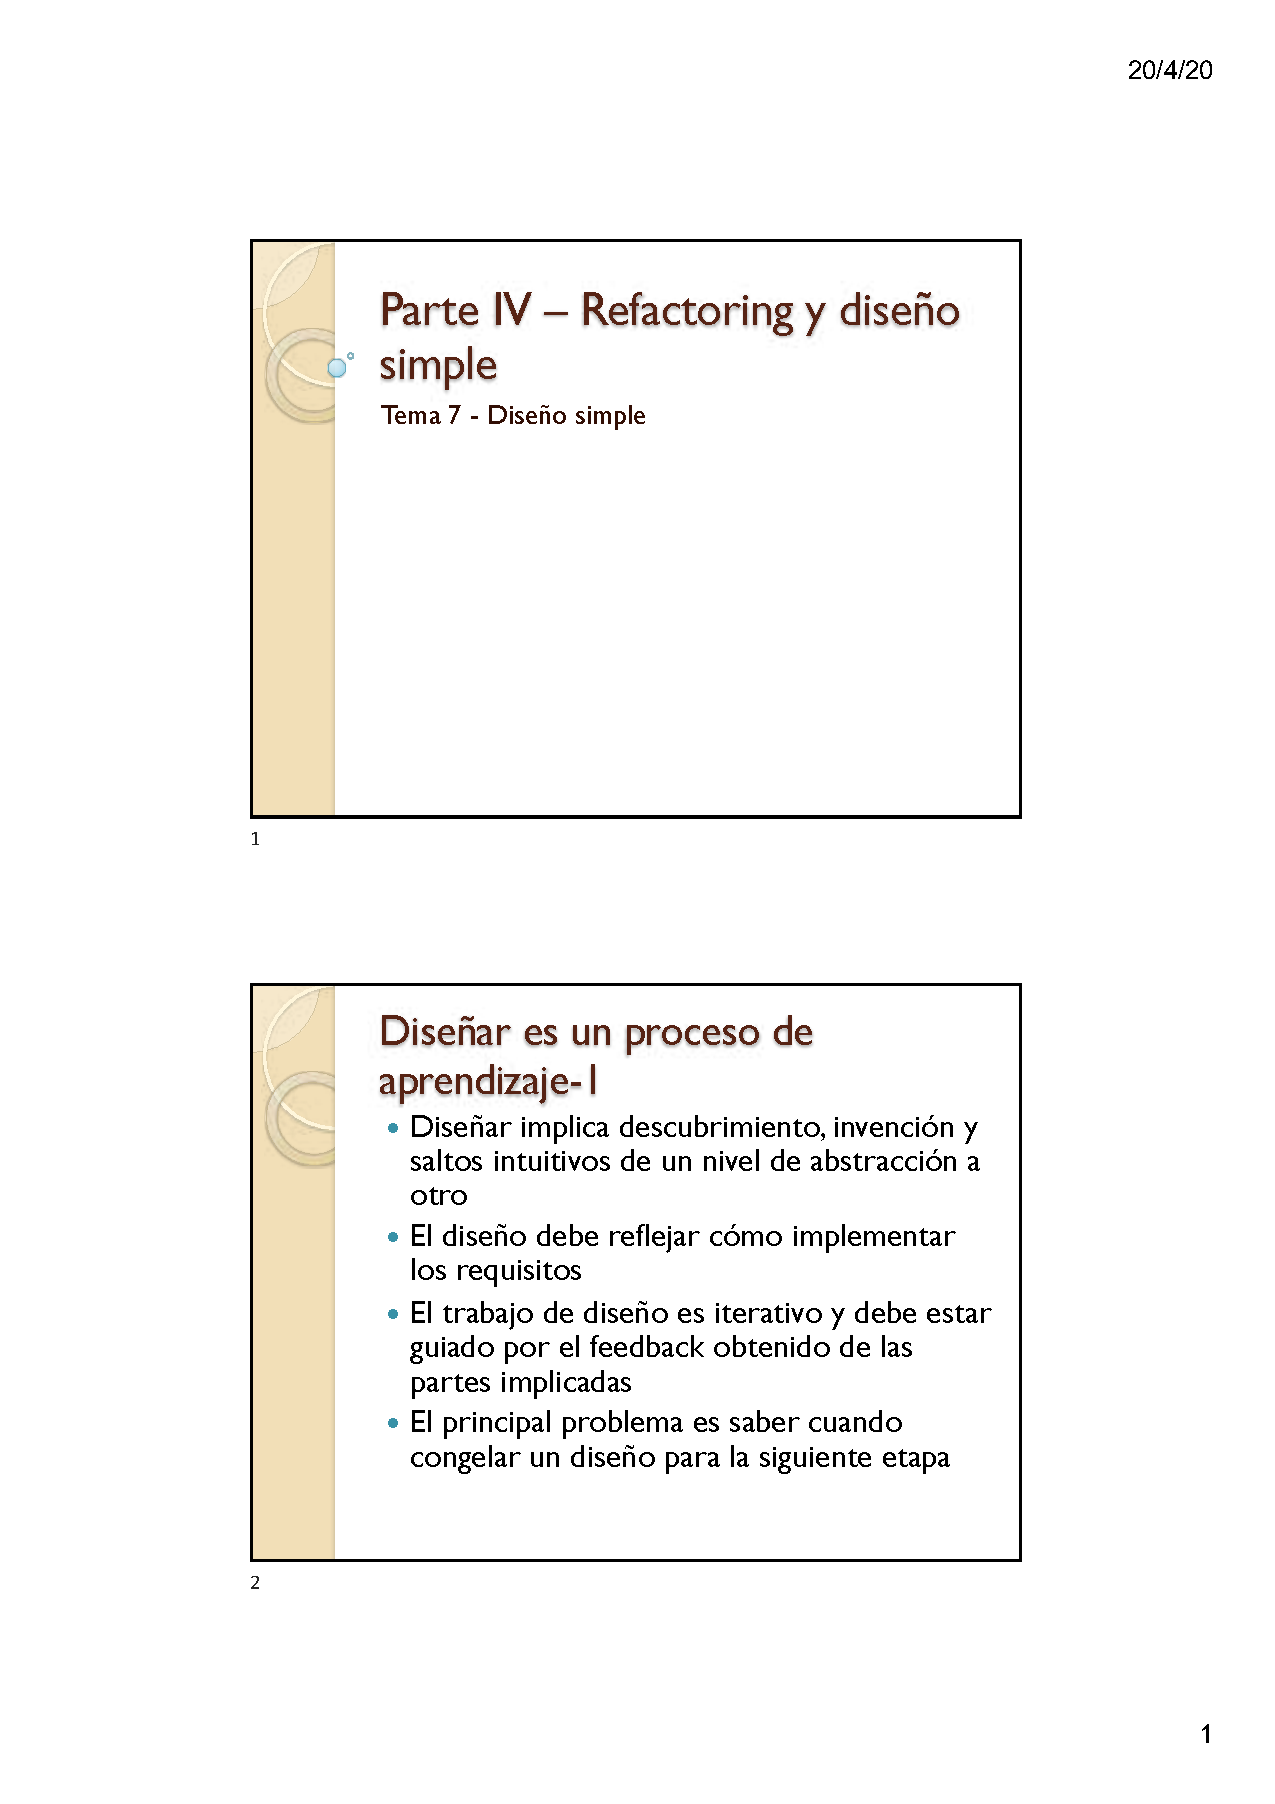
\includepdf[pages=-]{docs/Tema_7_-_Diseno_simple_y_patrones.pdf}

\part{Teoría}

\includepdf[pages=-]{docs/Presentacion_1_-_Aspecto_eticos_y_profesionales.pdf}
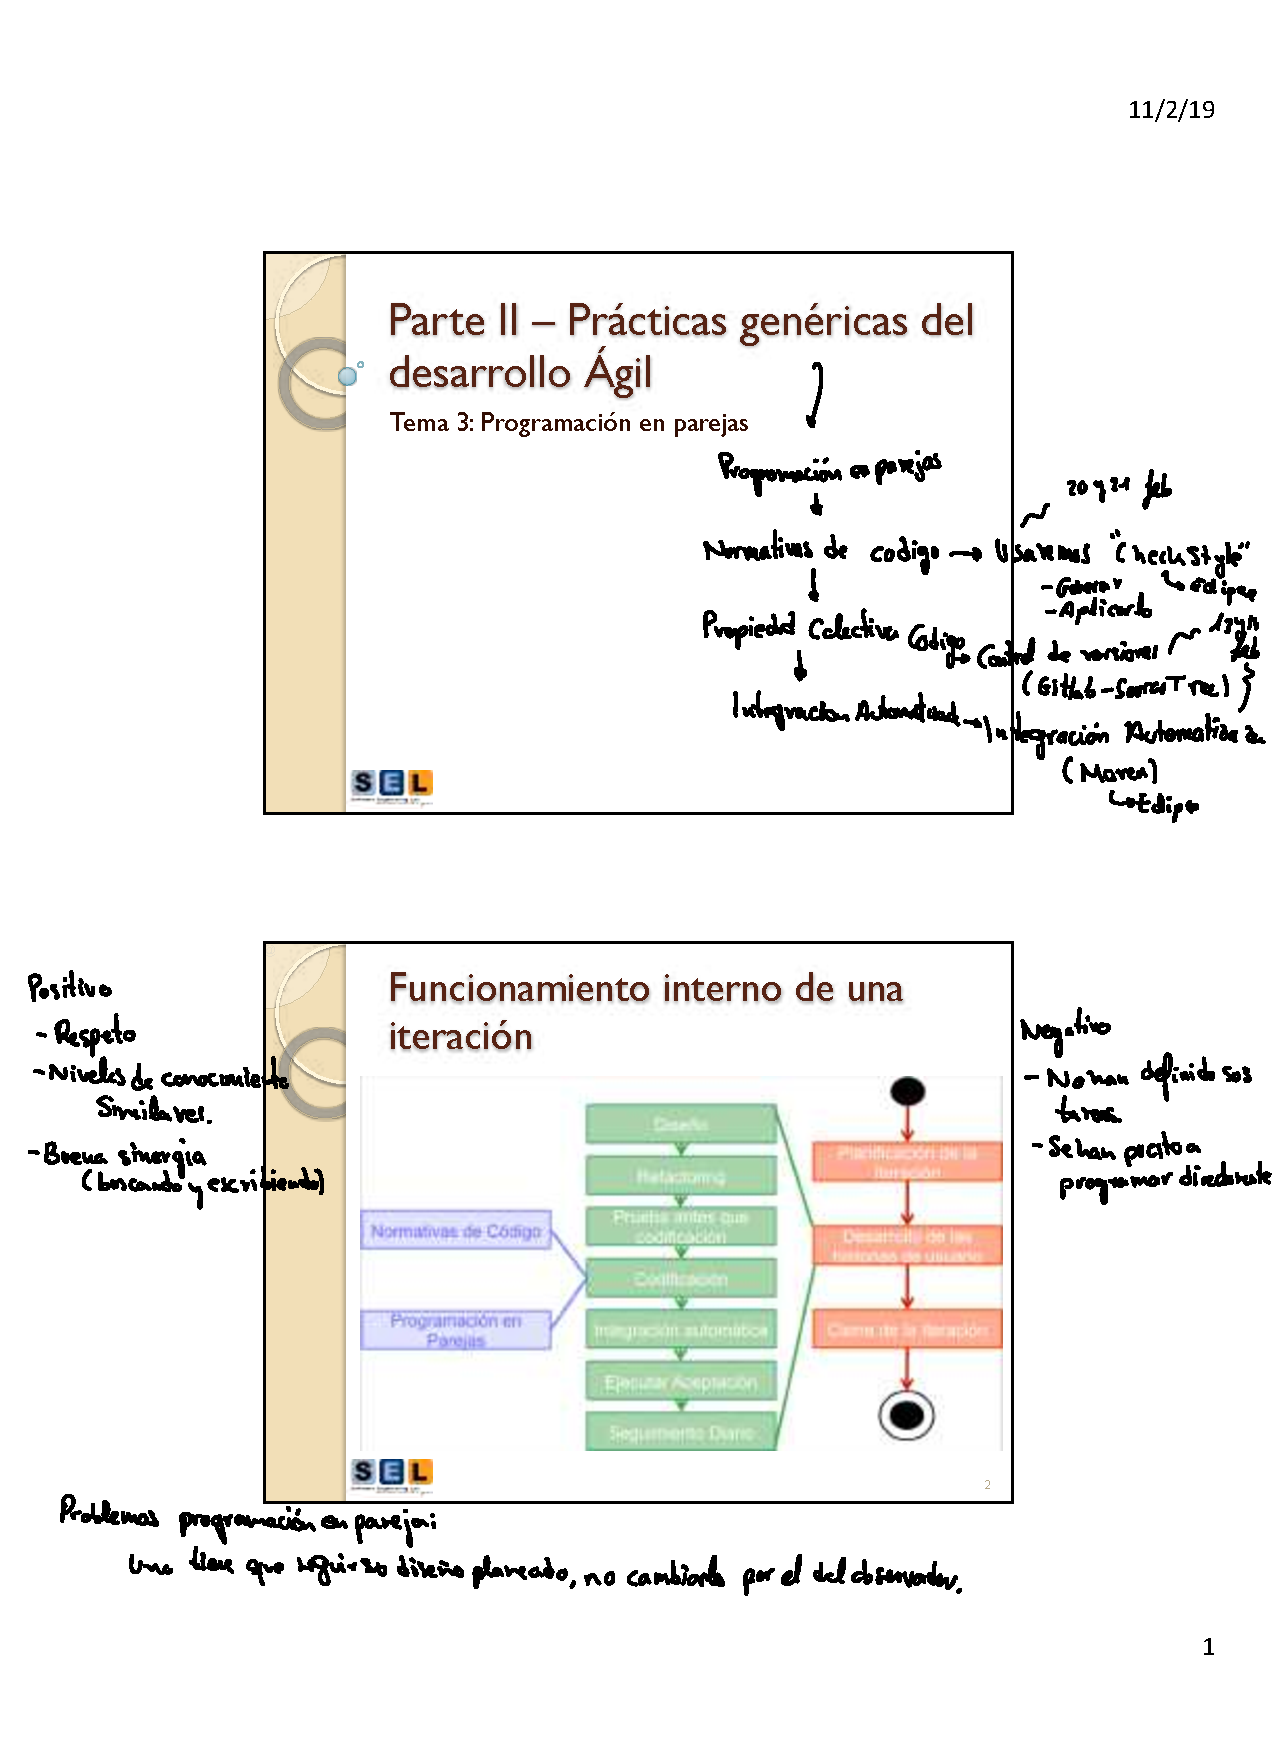
\includepdf[pages=-]{docs/Presentacion_2.1_-_Programacion_en_Parejas.pdf}
\includepdf[pages=-]{docs/Presentacion_2.2_-_Propiedad_Colectiva_de_Codigo.pdf}
\includepdf[pages=-]{docs/Presentacion_2.3_-_Normativas_de_Codigo.pdf}
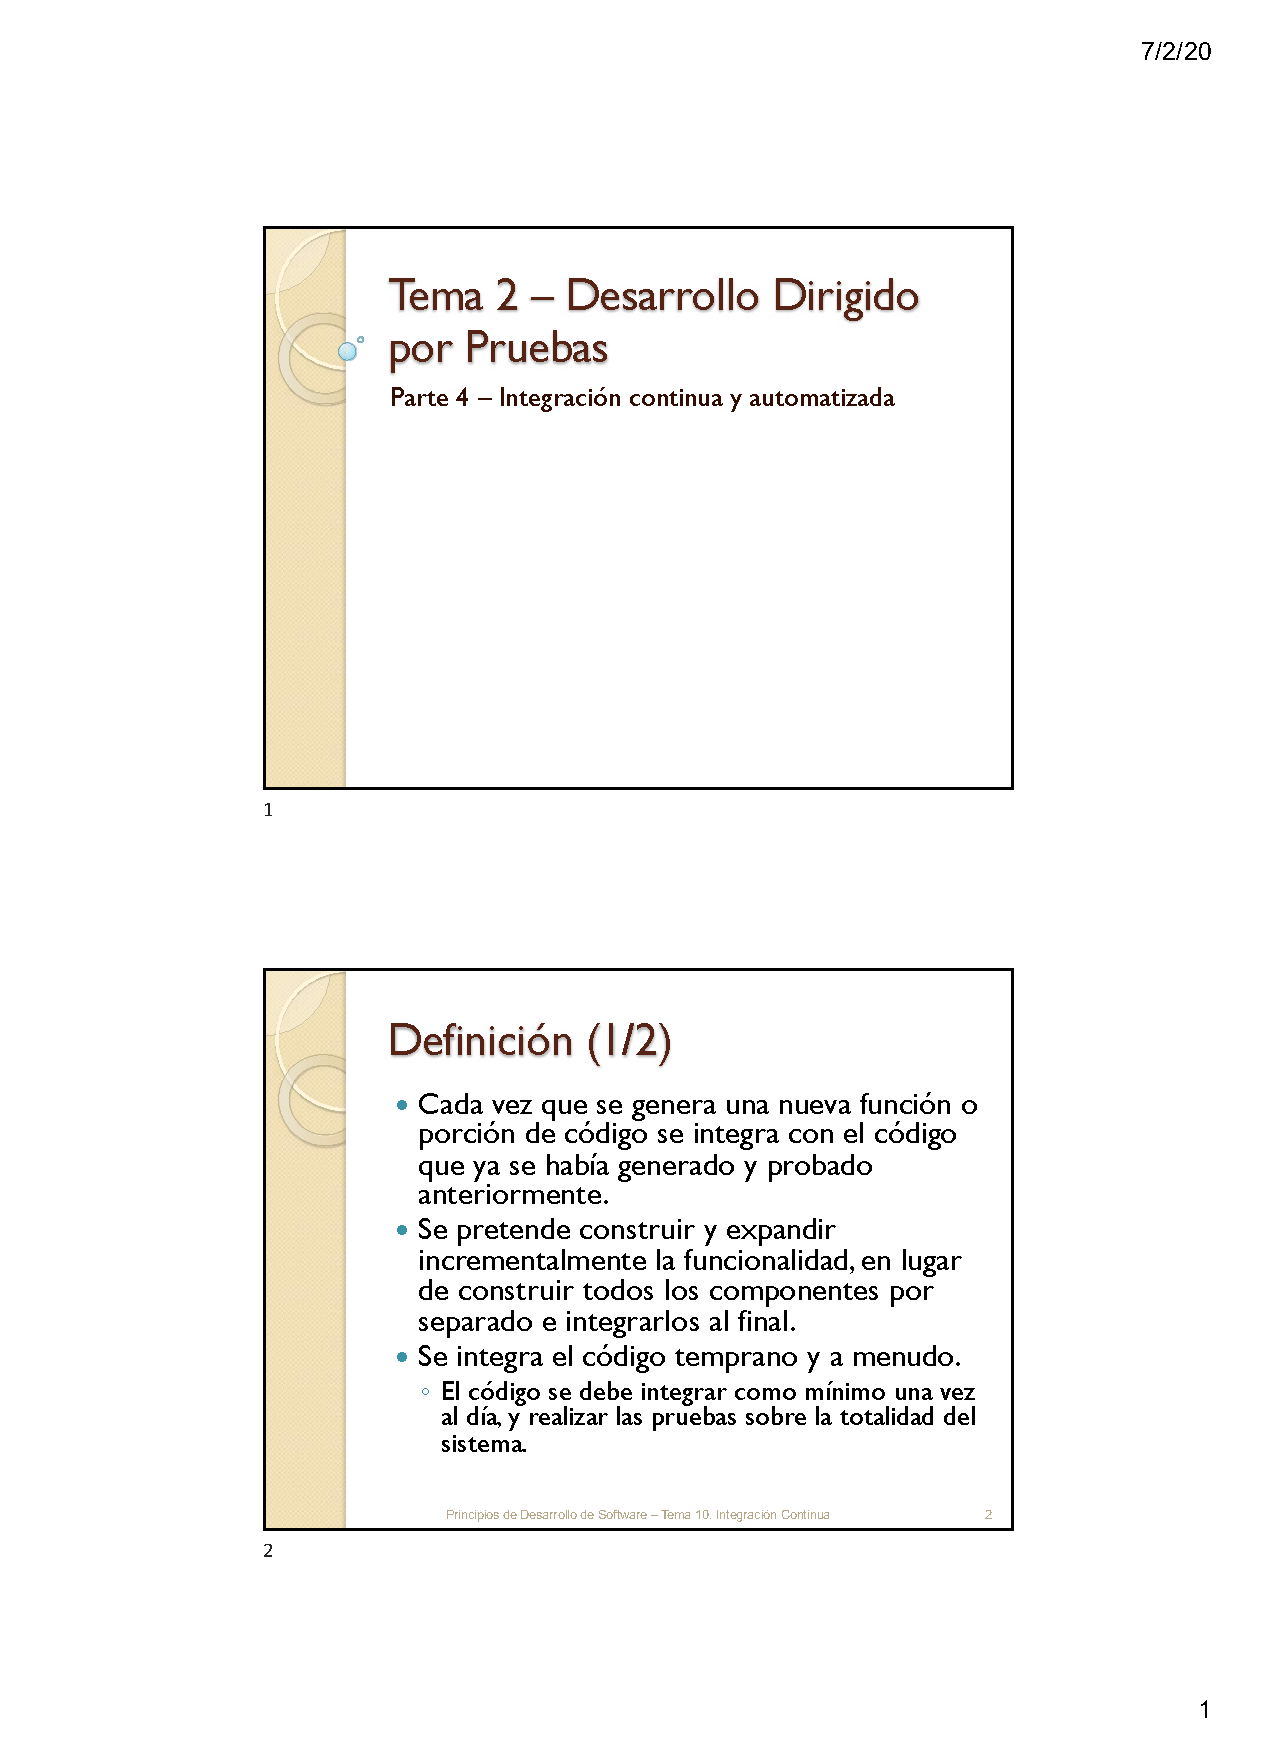
\includepdf[pages=-]{docs/Presentacion_2.4_-_Integracion_continua_y_automatizada.pdf}
\includepdf[pages=-]{docs/Presentacion_3_-_Principios_del_desarrollo_dirigido_por_pruebas.pdf}
\includepdf[pages=-]{docs/Presentacion_4_-_Analisis_Sintactico.pdf}
\includepdf[pages=-]{docs/Presentacion_4_-_Pruebas_funcionales_PA_y_BVA.pdf}

\part{Lecturas}
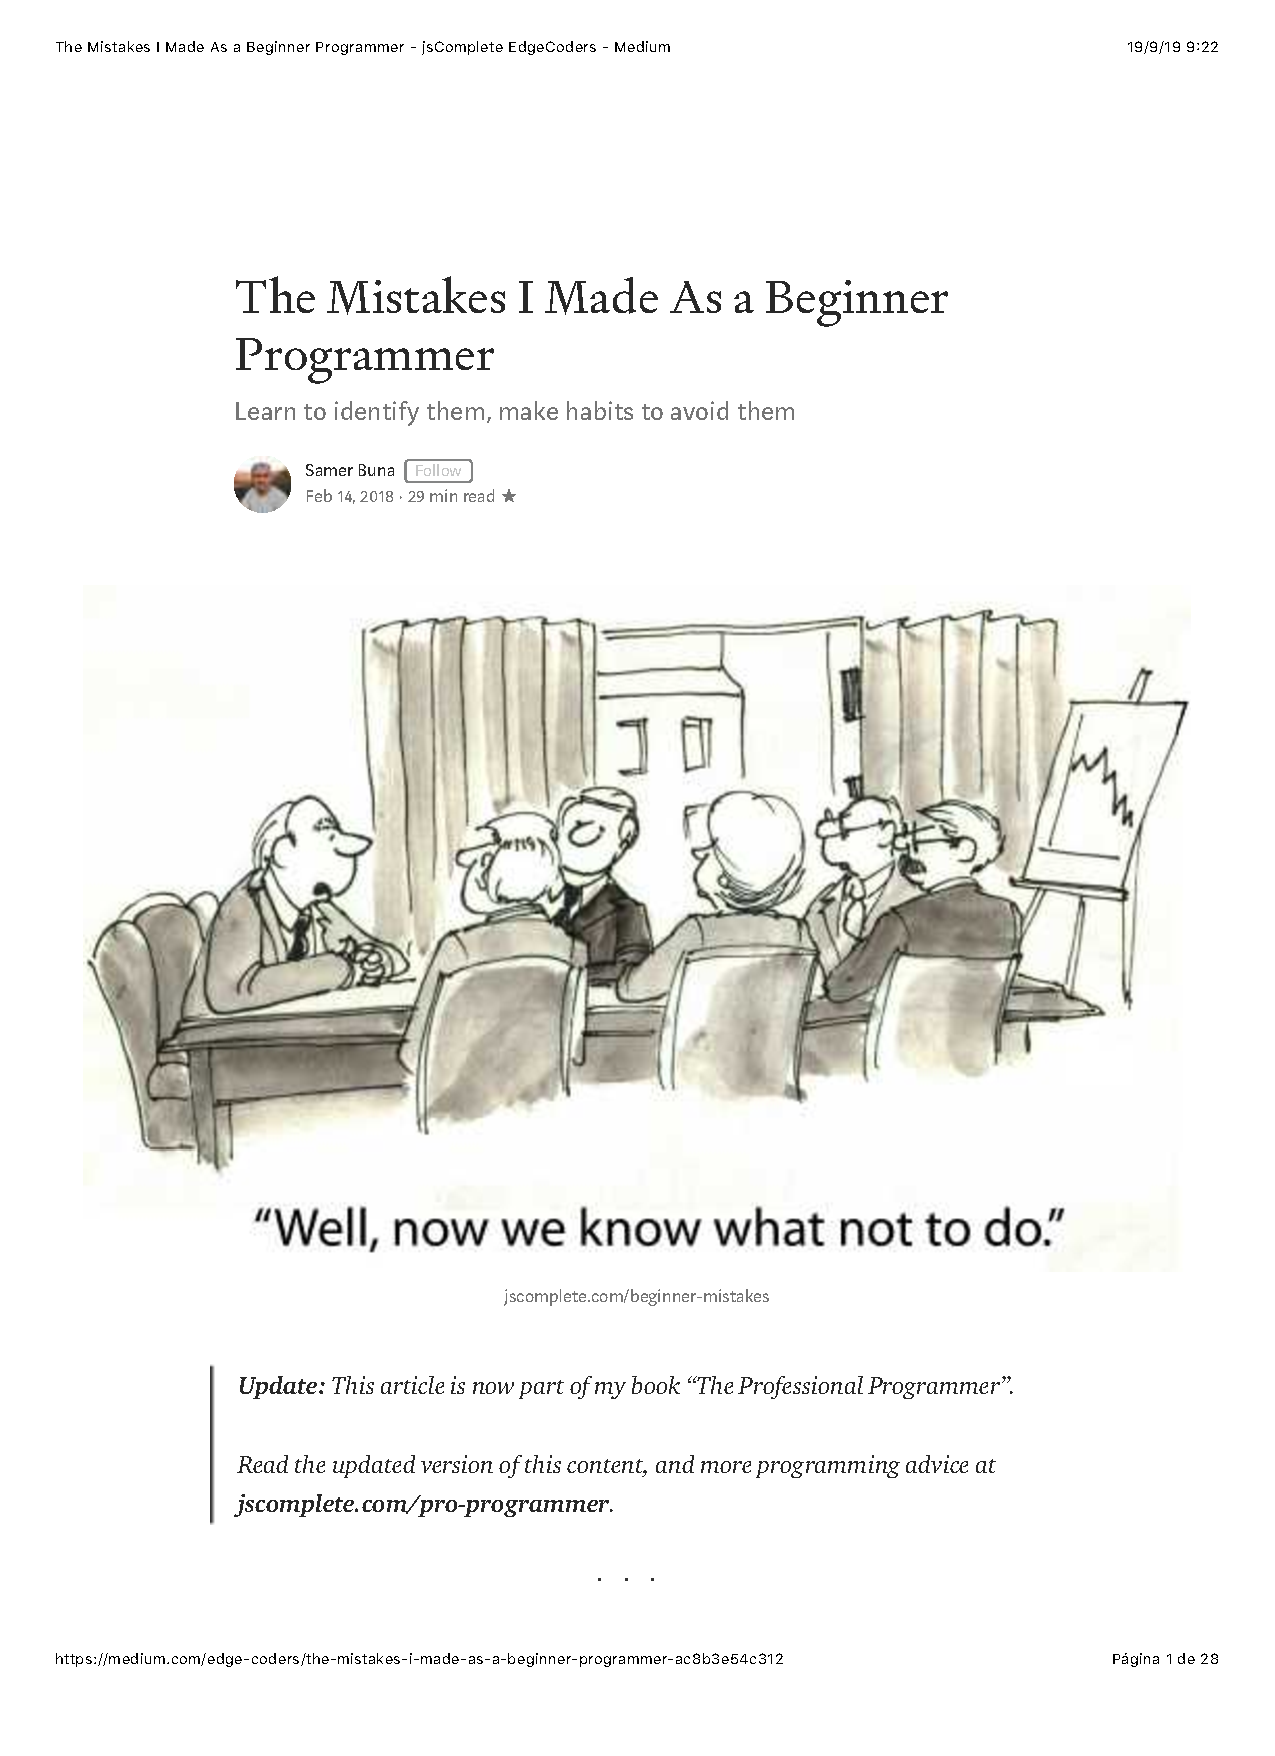
\includepdf[pages=-]{docs/Lectura_1_The_Mistakes_I_Made_As_a_Beginner_Programmer_-_jsComplete_EdgeCoders_-_Medium.pdf}
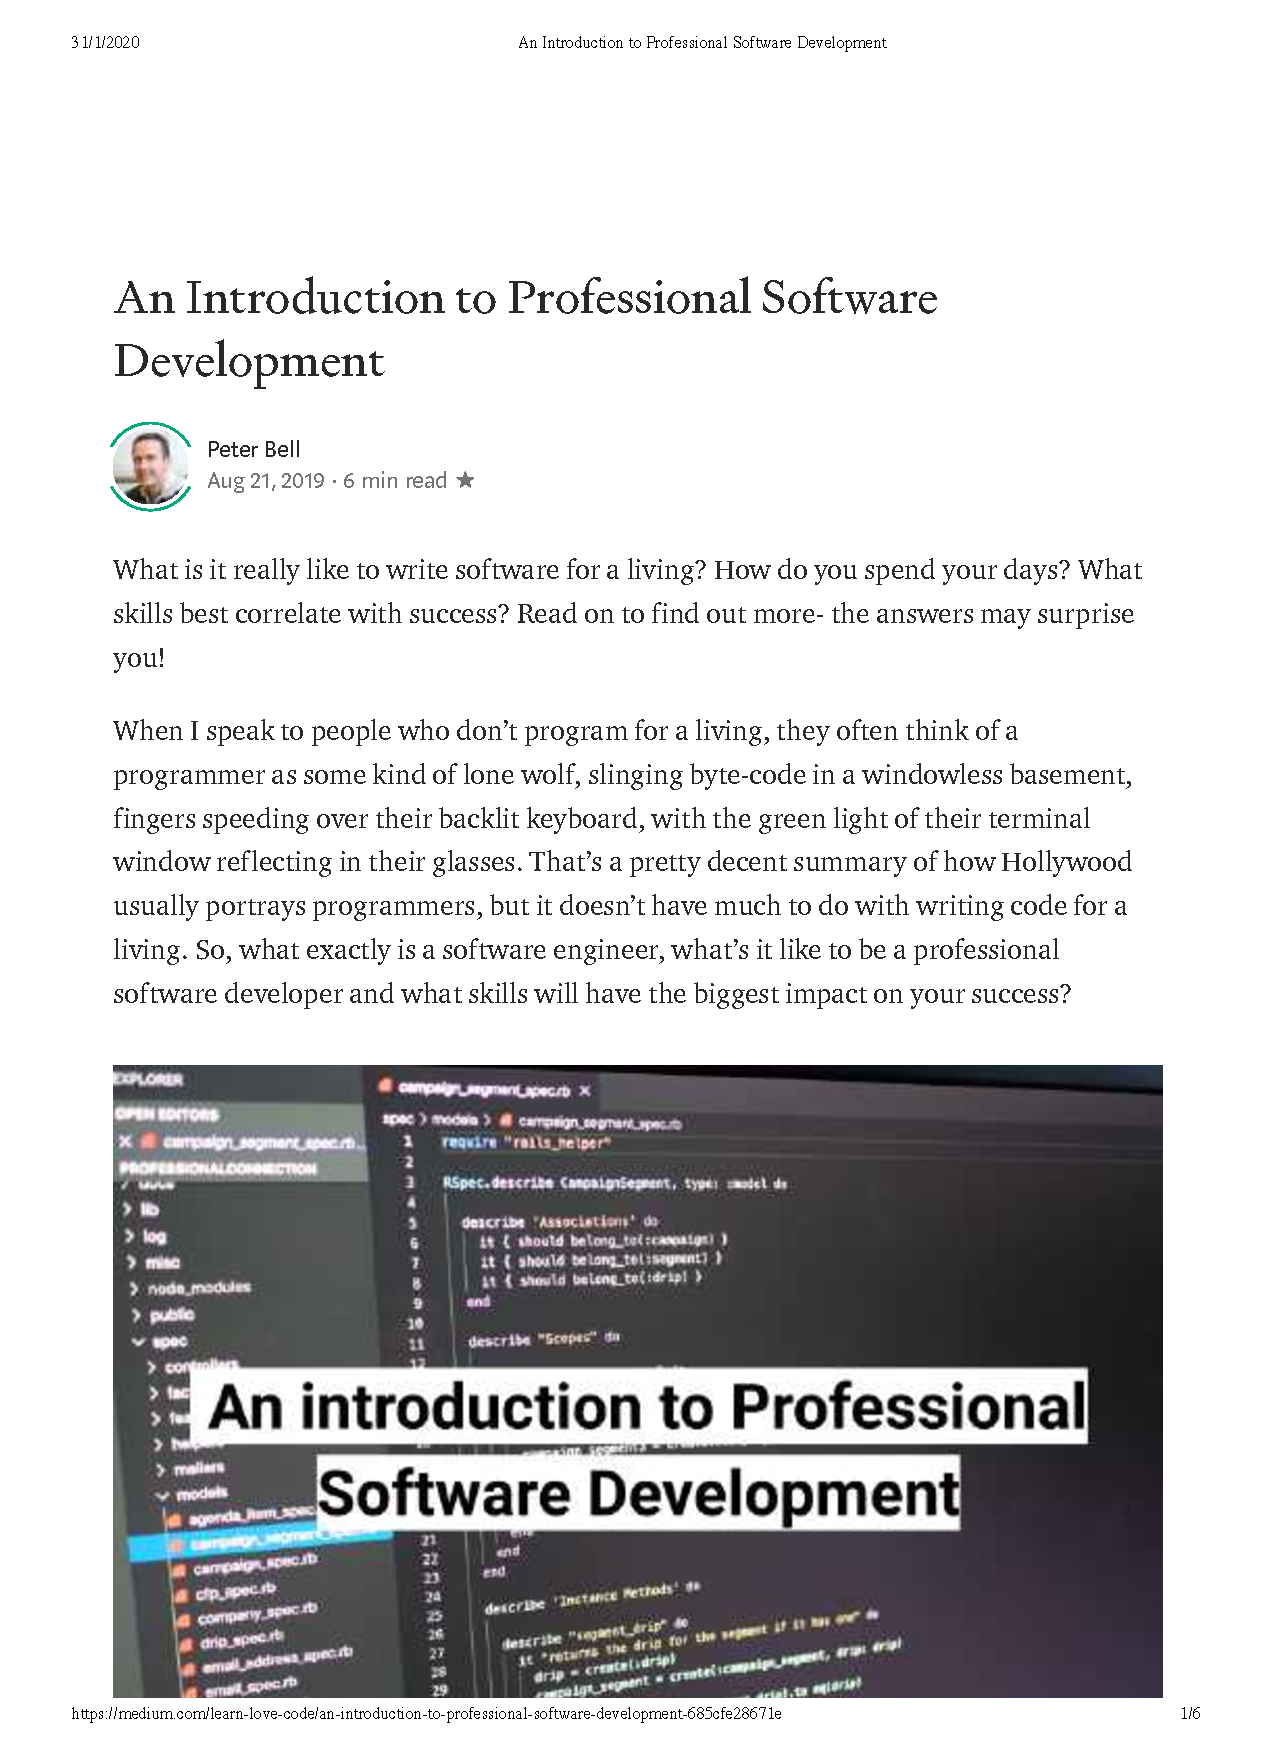
\includepdf[pages=-]{docs/Lectura_2_An_Introduction_to_Professional_Software_Development.pdf}
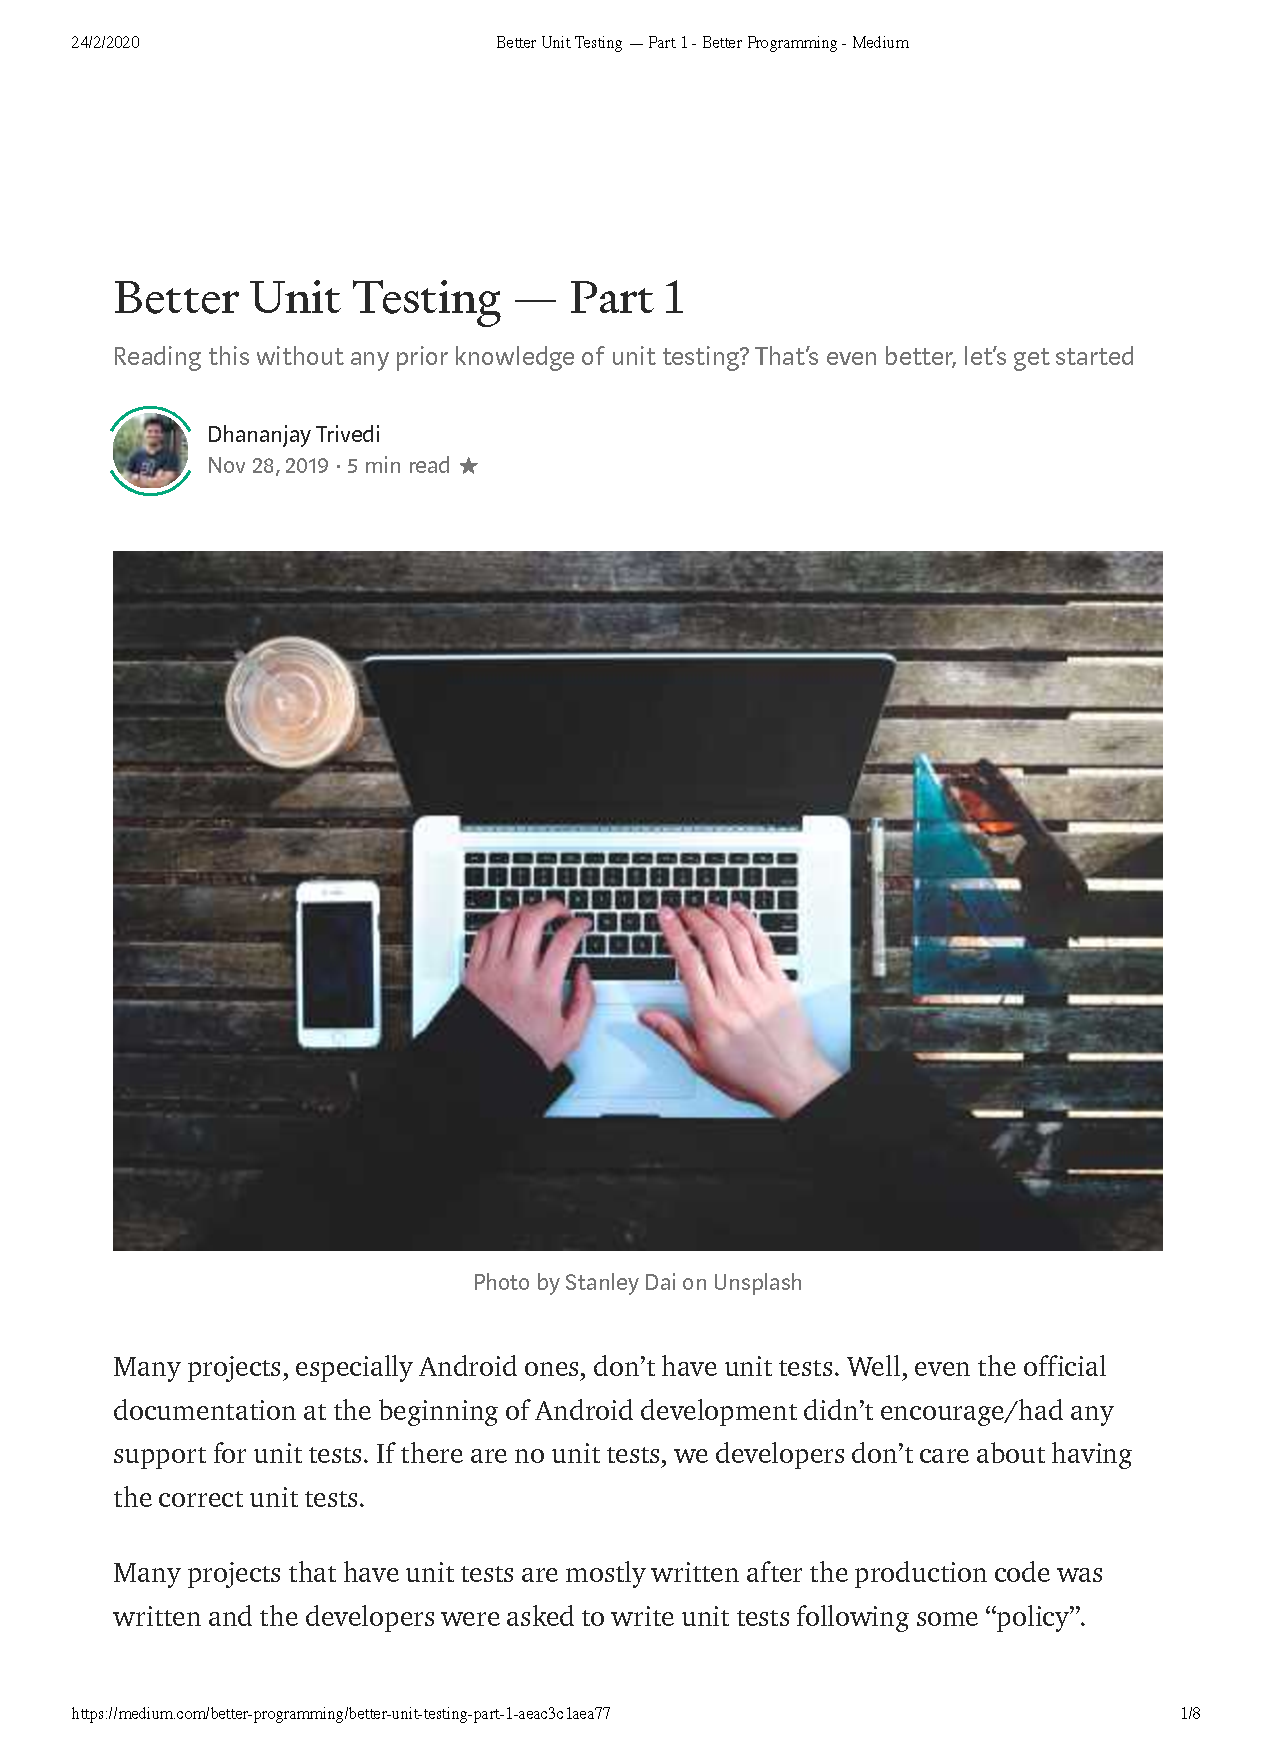
\includepdf[pages=-]{docs/Lectura_3_Better_Unit_Testing__Part_1_-_Better_Programming_-_Medium.pdf}
\includepdf[pages=-]{docs/Lectura_3_Better_Unit_Testing_(Part_2)_-_Better_Programming_-_Medium.pdf}
\includepdf[pages=-]{docs/Lectura_3_TDD__Lets_Take_a_Deep_Dive_-_The_Startup_-_Medium.pdf}
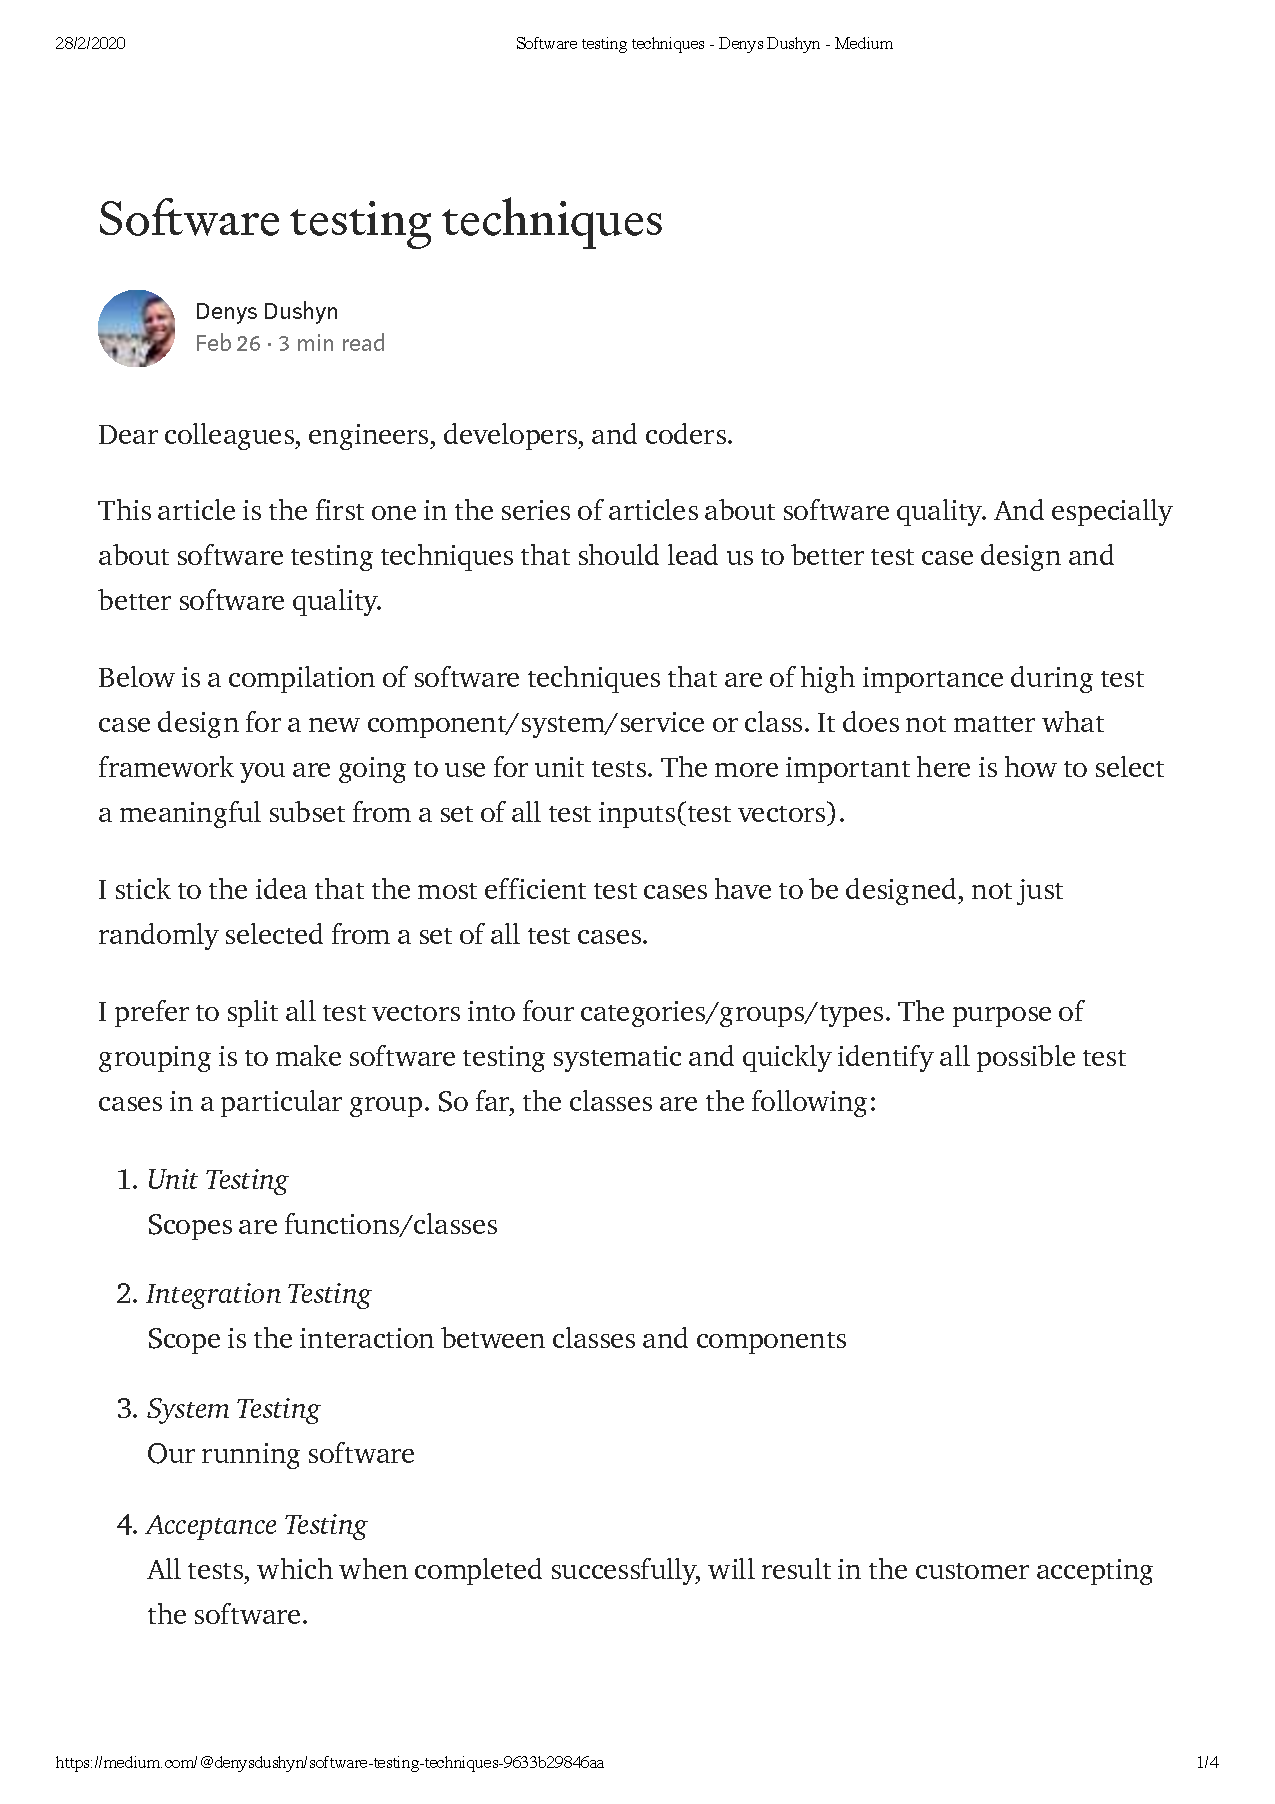
\includepdf[pages=-]{docs/Lectura_4_Software_testing_techniques_-_Denys_Dushyn_-_Medium.pdf}
\includepdf[pages=-]{docs/Lectura_4_Software_Testing__Difference_Between_Equivalence_Partitioning_and_BVA.pdf}

\part{Ejercicio guiado 1}

\includepdf[pages=-]{docs/Ejercicio2_100405951_100405834.pdf}

\includepdf[pages=-]{docs/Ejercicio1_100405951_100405834.pdf}

\includepdf[pages=-]{docs/Ejercicio_1_-_Enunciado.pdf}
\includepdf[pages=-]{docs/Code_of_Ethics.pdf}

\part{Ejercicio guiado 2}

\includepdf[pages=-]{docs/Ejercicio_Guiado_2_-_Enunciado.pdf}
\includepdf[pages=-]{docs/Normativa_de_cdigo.pdf}

\part{Ejercicio guiado 3}

\includepdf[pages=-]{docs/Memoria.pdf}

\includepdf[pages=-]{docs/Ejercicio_3_-_Enunciado.pdf}
\includepdf[pages=-]{docs/Ejercicio_Guiado_3_-_Sesion_2.pdf}
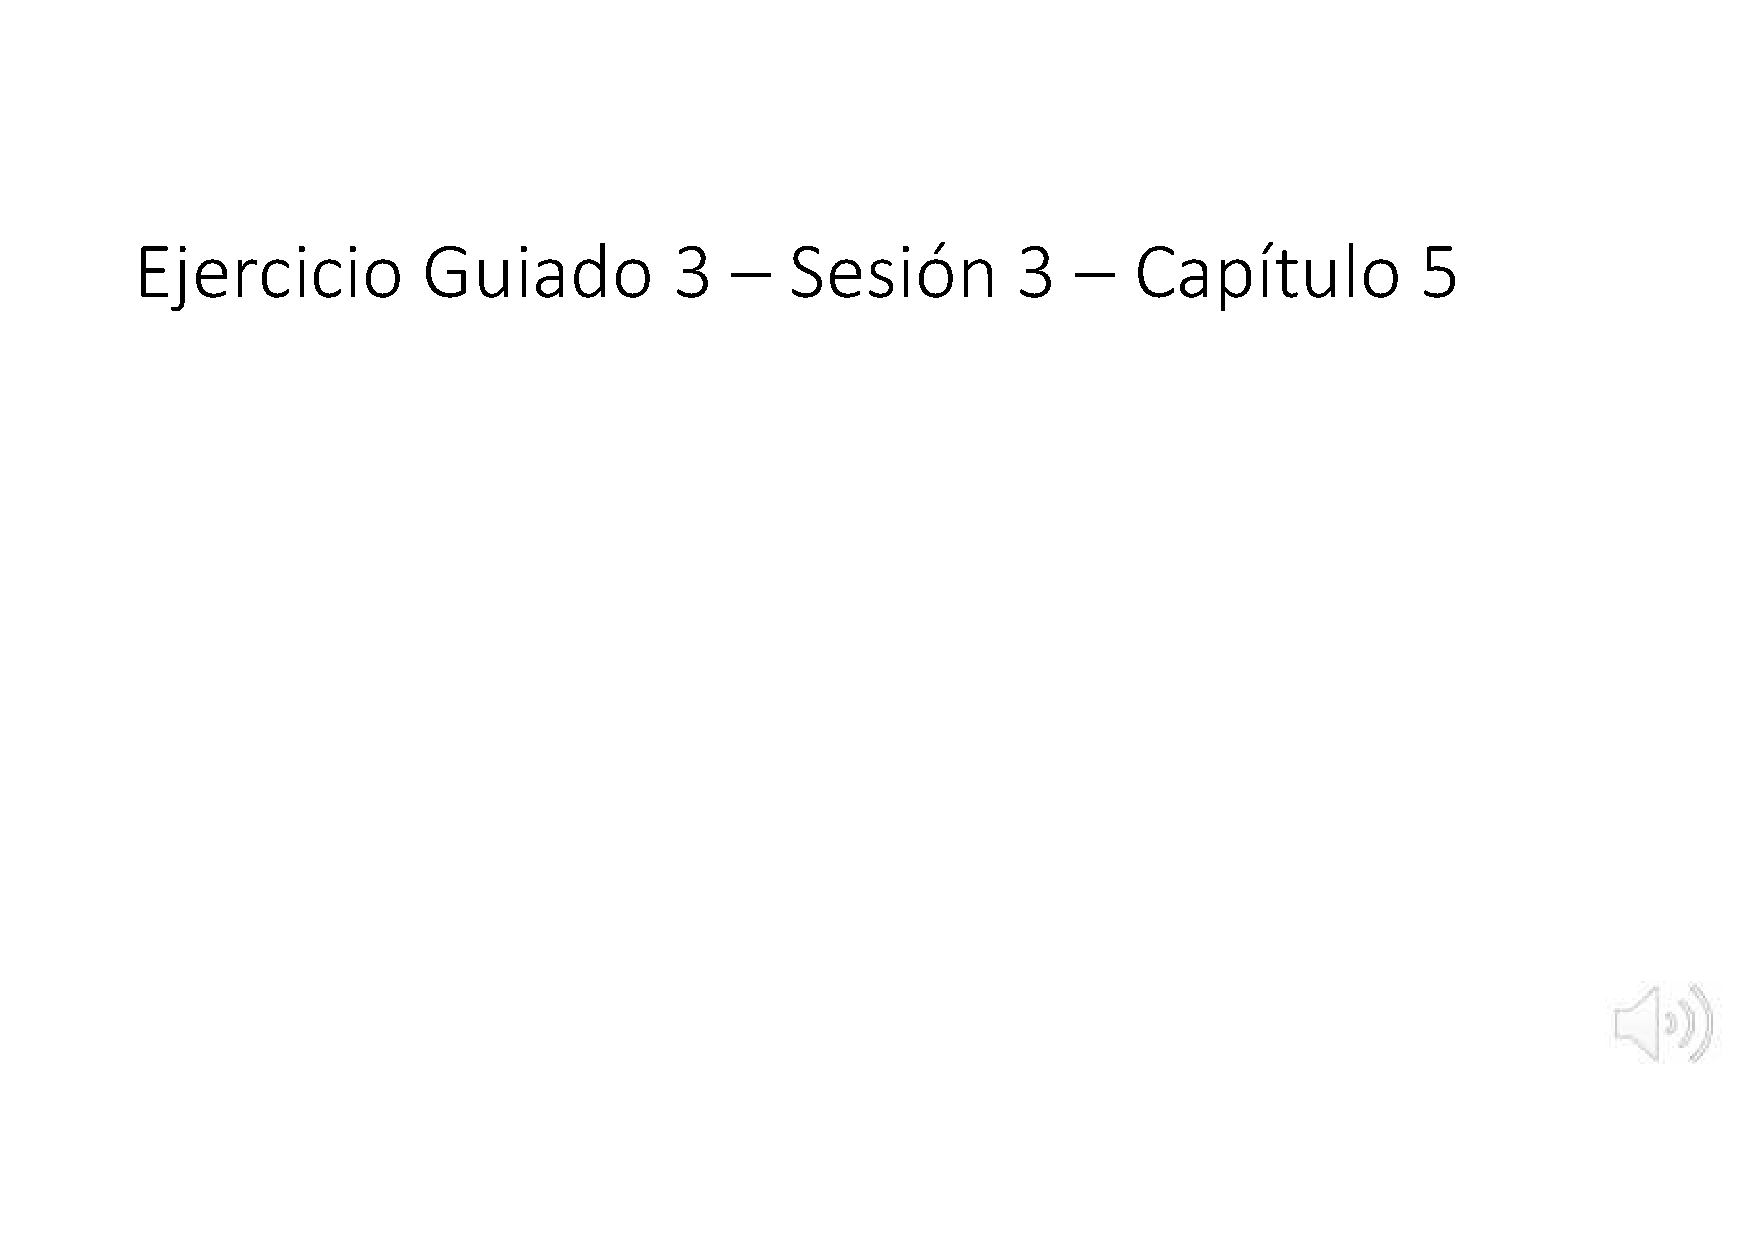
\includepdf[pages=-]{docs/Ejercicio_Guiado_3_-_Sesion_3.pdf}
\includepdf[pages=-]{docs/Normativa_de_cdigo.pdf}
\includepdf[pages=-]{docs/Presentacion_JUnit_2020_v4.pdf}

\part{Ejercicio guiado 4}
\includepdf[pages=-]{docs/Ejercicio_Guiado_4.pdf}

\part{Ejercicios clase}

\includepdf[pages=-]{docs/Ejercicio_3_-_Enunciado.pdf}
\includepdf[pages=-]{docs/Ejercicio_Guiado_3_-_Sesion_2.pdf}

\includepdf[pages=-]{docs/Practica_1_PDS.pdf}

\includepdf[pages=-]{docs/Practica_2_PDS.pdf}
\includepdf[pages=-]{docs/Presentacion_JUnit_2020_v4.pdf}
\includepdf[pages=-]{docs/Tema_1_-_Ejercicios_Clase.pdf}

\part{Practica final}

\includepdf[pages=-]{docs/Memoria.pdf}

\includepdf[pages=-]{docs/Practica_Final_-_Enunciado.pdf}

\part{Recursos}
\includepdf[pages=-]{docs/218.15972.pdf}

\end{document}